\documentclass[tikz, border=5pt]{standalone}
\usepackage{tikz}
\usepackage[dvipsnames]{xcolor}
\usetikzlibrary{calc, positioning}

\begin{document}
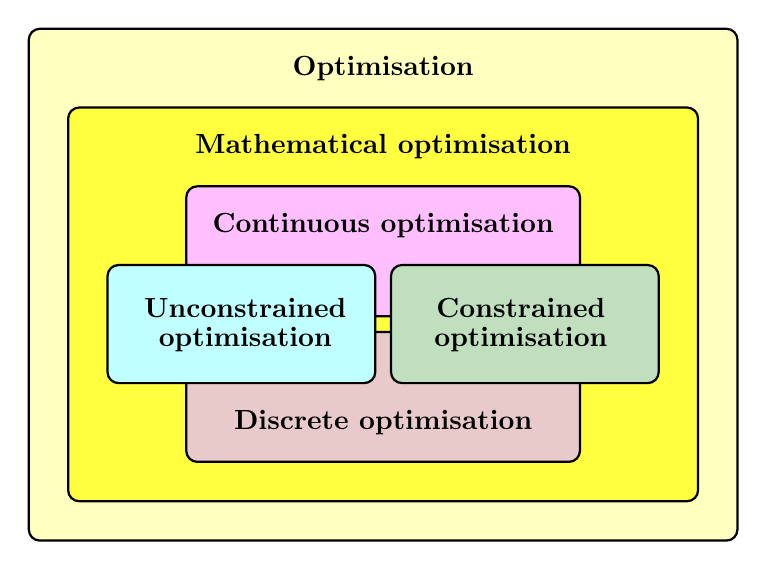
\begin{tikzpicture}[
        thick,
        draw=black,
        rounded corners,
        font=\bfseries,
    ]

    \def\xleft{0}
    \def\xright{9}
    \def\ytop{0}
    \def\ybottom{-6.5}
    \def\h{1.75}

    \pgfmathsetmacro{\xmid}{(\xleft+\xright)/2}
    \pgfmathsetmacro{\ymid}{(\ytop+\ybottom)/2}

    \filldraw[fill=Yellow!25]
    (\xleft,\ytop) rectangle (\xright,\ybottom);
    \node at (\xmid,\ytop-0.5) {Optimisation};

    \filldraw[fill=Yellow!75] (\xleft+0.5,\ytop-1) rectangle (\xright-0.5,\ybottom+0.5);
    \node at (\xmid,\ytop-1.5) {Mathematical optimisation};

    \filldraw[fill=Magenta!25] (\xleft+2,\ytop-2) rectangle (\xright-2,\ytop-2-\h+0.1);
    \node at (\xmid,\ytop-2.5) {Continuous optimisation};

    \filldraw[fill=Brown!25] (\xleft+2,\ybottom+1+\h-0.1) rectangle (\xright-2,\ybottom+1);
    \node at (\xmid,\ybottom+1.5) {Discrete optimisation};

    \filldraw[fill=Cyan!25] (\xleft+1,\ytop-3) rectangle (\xmid-0.1,\ybottom+2);
    \node at (\xleft+\xmid/2+0.5,\ymid-0.5+0.2) {Unconstrained};
    \node at (\xleft+\xmid/2+0.5,\ymid-0.5-0.2) {optimisation};

    \filldraw[fill=Green!25] (\xmid+0.1,\ytop-3) rectangle (\xright-1,\ybottom+2);
    \node at (\xright-\xmid/2-0.5,\ymid-0.5+0.2) {Constrained};
    \node at (\xright-\xmid/2-0.5,\ymid-0.5-0.2) {optimisation};

\end{tikzpicture}
\end{document}
